\documentclass[12pt,a4paper]{report}
\usepackage[utf8]{inputenc}
\usepackage[english]{babel}
\usepackage{amsmath}
\usepackage{amsfonts}
\usepackage{amssymb}
\usepackage[table,xcdraw]{xcolor}
\usepackage{graphicx}
\usepackage{amsmath}
\usepackage{fancyhdr}
\usepackage{cite}
\usepackage{framed}
\usepackage{a4wide}
\usepackage{float}
\linespread{1.5}
\usepackage{blindtext}
\setcounter{tocdepth}{2}
\usepackage{xpatch}
\makeatletter
\pagestyle{fancy}
\fancyhf{}
\setlength{\headheight}{15pt}  
\lhead{\small{\leftmark}}
\rhead{\rightmark}
\fancyfoot[CE,CO]{\thepage}
\renewcommand{\headrulewidth}{2pt}
\renewcommand{\footrulewidth}{2pt}
\usepackage[T1]{fontenc}

%centering chapter names

\xpatchcmd{\@makechapterhead}{%
  \huge \bfseries \@chapapp \space \thechapter
}{%
  \Large \bfseries\centering \MakeUppercase \@chapapp \space \thechapter
}{\typeout{Patched @makechapterhead}}{\typeout{Patching of @makechapterhead failed}}

\makeatother
%centering chapter names

\usepackage[utf8]{inputenc}
%\usepackage{fourier, erewhon, cabin}
\usepackage[english]{babel}
\usepackage{titletoc}
\addto\captionsenglish{ \renewcommand*\contentsname{\centerline{\large CONTENTS}}}


\titlecontents{chapter}
[5.5em] %5.3
{\bigskip}
{\contentslabel[\textsc{\small \chaptername}~\thecontentslabel]{5.5em}}%\thecontentslabel
{\hspace*{-5.5em}}% unnumbered chapters
{\titlerule*[0.5pc]{ }\contentspage}[\smallskip]%

\titlecontents{section}
[5.5em] % i
{\smallskip}
{\small \thecontentslabel\enspace}%\thecontentslabel
{\hspace*{-5.5em}}
{\titlerule*[0.5pc]{ }\contentspage}%]

\titlecontents{subsection}
[7.12em] %
{\smallskip}
{\thecontentslabel\enspace}%\thecontentslabel
{\hspace*{7.12em}}
{\titlerule*[0.5pc]{ }\contentspage}


\begin{document}
\pagestyle{empty}
\begin{center}
{\Large \textbf{ASIC for Navigation Application with Programmable Peripheral Logic}}\\
\vspace{0.2cm}
PROJECT REPORT\\
\vspace{0.2cm}
Submitted by \\
\vspace{0.2cm}
\textbf{MANJUSHA M}\\
\textbf{TVE16EC032}\\
\vspace{0.12cm}
\textbf{RAMDAS PRASAD H}\\
\textbf{TVE16EC040}\\
\vspace{0.12cm}
\textbf{SRUTHI SANTHOSH}\\
\textbf{TVE16EC051}\\
\vspace{0.12cm}
\textbf{to}\\
\vspace{0.12cm}
the A P J Abdul Kalam Technological University \\
in partial fulfillment of the requirements for the award of the Degree \\
of\\
Bachelor of Technology \\
In\\
\textit{Electronics and Communication Engineering}\\

\includegraphics[scale=0.4]{CET_logo.jpeg}\\
\textbf{Department of Electronics and Communication Engineering}\\
College of Engineering\\
Trivandrum\\
July, 2020
\end{center}
\newpage
\begin{center}
\textbf{\large DECLARATION}
\end{center}
We undersigned hereby declare that the project report ( “ASIC for Navigation Application with Programmable Peripheral Logic”) , submitted for partial fulfillment of the requirements for the award of degree of Bachelor of Technology of the APJ Abdul Kalam Technological University, Kerala is a bonafide work done by us under supervision of Prof. Lalu V. This submission represents our ideas in our own words and where ideas or words of others have been included, we have adequately and accurately cited and referenced the original sources. We also declare that we have
adhered to ethics of academic honesty and integrity and have not misrepresented or fabricated any data or idea or fact or source in our submission. We understand that any violation of the above will be a cause for disciplinary action by the institute and/or the
University and can also evoke penal action from the sources which have thus not been properly cited or from whom proper permission has not been obtained. This report has not been previously formed the basis for the award of any degree, diploma or similar title of any other University.\\
\noindent 
\begin{minipage}{0.45\linewidth}
\begin{flushleft}
\vspace{1 cm}
                         
Place \\
Date\\

\end{flushleft} 
\end{minipage}
\hfill
\begin{minipage}{0.45\linewidth}
\begin{flushright}                                      
\vspace{2cm}
Manjusha M\\
\vspace{2cm}                         
Ramdas Prasad H\\
\vspace{2cm}
Sruthi Santhosh\\


\end{flushright} 
\end{minipage}

\thispagestyle{empty}
\newpage
\begin{center}

%\vspace{1.5cm}

\textbf{DEPT. OF ELECTRONICS AND COMMUNICATION ENGINEERING}

\textbf{COLLEGE OF ENGINEERING}

\textbf{TRIVANDRUM}

\textbf{2019 - 2020}
\end{center}
\begin{center}

\includegraphics[scale=0.4]{CET_logo.jpeg}

\end{center}
\begin{center}
 \textbf{\large{CERTIFICATE}}
\end{center}
 
This is to certify that the report entitled \textbf{ \large ASIC for Navigation Application with Programmable Peripheral Logic} submitted by \textbf{Manjusha M, Ramdas Prasad H and Sruthi Santhosh}, to the APJ Abdul Kalam Technological University in partial fulfillment of the B.tech. degree in Electrical and Electronics Engineering is a bonafide record of the project work carried out by them under our
guidance and supervision. This report in any form has not been submitted to any other University or Institute for any purpose.

\noindent 
\begin{minipage}{0.35\linewidth}
\begin{flushleft}
\vspace{2 cm}
                         
\textbf{Project Coordinator} \\
\vspace{0.8cm}
Prof. Gijy P. G.\\
\footnotesize{Assistant Professor\\
Dept. of ECE.\\
College of Engineering\\
Trivandrum}\\
\end{flushleft} 
\end{minipage}
\begin{minipage}{0.35\linewidth}
\begin{center}
\vspace{2 cm}
                         
\textbf{Project Coordinator} \\
\vspace{0.8cm}
Prof. Lalu V.\\
\footnotesize{Assistant Professor\\
Dept. of ECE.\\
College of Engineering\\
Trivandrum}\\
\end{center} 
\end{minipage}
\begin{minipage}{0.35\linewidth}
\begin{flushright}                                      
\vspace{2cm}                         
\textbf{Head of the Department} \\
\vspace{.8cm}
Dr. Santhosh Kumar S.\\
\footnotesize{Professor\\
Dept. of ECE.\\
College of Engineering \\
Trivandrum}\\
\end{flushright} 
\end{minipage}
\thispagestyle{empty}

\chapter*{\centering \large ACKNOWLEDGEMENT\markboth{Acknowledgements}{Acknowledgements}}


 We take this opportunity to express our deep sense of gratitude and sincere thanks to all who helped us to complete the work successfully. Our first and foremost thanks go to God Almighty who showered in immense blessings on our effort.

 We wish to express our sincere thanks to \textbf{ Dr. Jiji C. V., Principal, College of Engineering, Trivandrum} for providing  us with all the necessary facilities and support.
 
 We would like to express our sincere gratitude to \textbf{Dr. Santhosh Kumar S (Head of the department)}, for his support and co-operation. 
 We wish to express our sincere gratitude towards all the teaching and non teaching staff members of our Department.
 
 Finally We thank our parents, all our friends, near and dear ones who directly and indirectly contribute to the successful completion of this work.




\begin{flushright}
\textbf{Manjusha M\\
Ramdas Prasad H\\
Sruthi Santhosh}
\end{flushright}
\pagenumbering{roman}
\addcontentsline{toc}{chapter}{ACKNOWLEDGEMENT}
\thispagestyle{empty}
\newpage
\chapter*{\centering \large ABSTRACT\markboth{Abstract}{Abstract}}
\addcontentsline{toc}{chapter}{ABSTRACT}
Systems designed for navigation require processing of real-time and conventional computing. This implies that the control hardware must be easily customizable, easy to debug, reliable and capable of handling real-time data, which may change depending on the application. These constraintsare typically met through two seperate solutions. A microcoontroller to handle control tasks and an FPGA to handle rela-time data. This is the optimal solution to the problem and is the the most widely accepted solution that currently exists. This project aims to integrate these two solutions onto a single Application Specific Integrated Circuit(ASIC) that meets all requirements. The Compute core, and programmable peripherals will be built up from scratch, along with essential core peripherals like UART and MIL-1553-STD. All other necessary protocols will be sourced from FPGA/ASIC proven open source, wishbone compatible peripherals. The aim of this project is create a roadmap for this special class of ASICs that have great value for the military as well as scientific application.
\newpage
\tableofcontents
\listoftables
\addcontentsline{toc}{chapter}{LIST OF TABLES}
\listoffigures
\addcontentsline{toc}{chapter}{LIST OF FIGURES}

\chapter{\large INTRODUCTION}
\pagenumbering{arabic}
\section{\small\MakeUppercase{General Background}}
\paragraph{\textrm{\textmd{Many real time applications where control Systems are utilized benefit from having hardware that can handle real time data. In situations where large-scale production of Application Specific Integrated Circuits (ASICs) for each and every problem situation is not feasible most conventional design requirements are met using Field Programmable Gate Arrays (FPGAs). This approach yields the benefit of the same template hardware boards to be reconfigured as per the specific application, even on the fly and give considerable flexibility to the platform while also contributing heavily to the considerable cost of the overall design. Hence for applications like Navigation systems for satellites the benefits of both approaches can be combined to create an ASIC which includes a processing core, multiple configurable logic blocks, support for standard IO interface standards and protocols and ADC/DACs, all on the same silicon. This allows considerable benefits to help tailor custom hardware, specific to the needs where the system is to deployed while allowing for the reliability and cost-effectiveness of Large scale production of ASICs in house.}}}
\paragraph{\textrm{\textmd{RISC-V is an Open-Source, frozen, Instruction-set Architecture (ISA), initially developed at The University of California, Berkeley. The ISA is a becoming a vastly popular alternative to CISC architectures and proprietary popular RISC architectures like ARM. The applications the system will encouter warrants the use of RISCV32-IM, which is the integer operation base 32 bit variant of the RISC-V ISA, with the multiply/divide extension.The processing core should preferably be pipelined and have necessary hazard detection and mitigation schemes.}}}
\paragraph{\textrm{\textmd{The inclusion of FPGA Blocks on the die presents unique software and hardware challenges that require adapting known standard solutions to function in the unique environment the ASIC design creates.These include adapting bus standards for ease of communication with and programming of the FPGA. Establishing optimal routing for the given FPGA architecture and automating the process of synthesizing a design on the FPGA blocks using the processing core, handling and generation of multiple clock domains internally and ability for the SoC to drive output pins  to different output voltage standards according to the application. This also brings about the need for an integrated onboard or external power management solution and multiple IO voltage domains. The project aims to create a unique ASIC that currently does not exist in the market and can find application in multiple domains. }}}
\section{\small \MakeUppercase{Objective}}
\section{\small \MakeUppercase{Scope}}
The project will have four different goals to achieve based on the ideas presented in the preceeding section. Firstly, Design a usable RISC-V compute core that is flexible and light-weight. Secondly implement the Programmable FPGA cores and implement a programming scheme. and then implement the necessary peripherals. Thirdly, synthesise and test the SoC elements on an FPGA and lastly, tapeout and fabrication. All elements of the SoC will be written in chisel and exported to verilog. Verilator can be used to test the SoC at the verilog level and exported to the tapeout tools available at the IISU before final fabrication.
\section{\small \MakeUppercase{Scheme of Project Work}}
\paragraph{\textrm{\textmd{
			The RISC-V Instruction-set Architecture is highly pipelining friendly as well as being comparatively easier to implement in hardware than nore conventional RISC ISAs like MIPS. This enables the design of a fast, minimalistic, pipelined compute core that can easily work as a backbone for the additional components necessary to meet the application requirements. It follows that a flexible yet simple FPGA architecture needs to be identified keeping in mind both the ease of ease of implementation and ease of programming it by the core. The Navigation ASIC will encounter both Real-Time Data and Complex Decision making tasks. Hence the compute core and the FPGA elements have distict roles to play in the ASIC. The FPGA block can be programmed to have Logic that handles the real time data while the compute core can handle less time-constrained tasks. To take it one step further the FPGA can be programmed on the fly by the compute core, thus ensuring better flexibility for the ASIC as well as making it much more of a powerful solution, eventhouh the individual components are not by any stretch, new architectural elements.}}}
\section{Constraints}
\paragraph{\textrm{\textmd{The proposed SoC should contain the following elements:}}}
\begin{itemize}
	\item RISC-V ISA processor with a five stage pipeline, hazard detection and avoidance
	\item UART, SPI(boot and programming through this interface), I2C, MIL-STD 1553 encoder decoder.
	\item On-board ADC and DAC interfaces. 
	\item Core Configurable FPGA Logic Blocks with multiple clock domain routing.
	\item Pin Drive Circuitry and Voltage level shifting.
\end{itemize}
\section{Proposed process}
\paragraph{\textrm{\textmd{According to the resources available the preffered HDL for design has been determined to be a combination of verilog and chisel. The design will be tested on an FPGA and once validated the design can be prepared for layout and fabrication. The rest of the project will be implemented using the Cadence Software Toolchain. The design process can be summarized in the following steps:}}}
\begin{enumerate}
	\item Creating a behavioural model of the ASIC in verilog using Chisel.
	\item Testing the design using a Verilog simulator like verilator.
	\item Exporting the design to FPGA and testing the ASIC subcomponents.
	\item Exporting the design to Cadence toolchain for onboarding and layout tasks.
	\item Preparing ASIC for fabrication using SCL 180nm as the target and testing.
	\item Mask generation and fabrication.
\end{enumerate}
%\section{Timeline}
%  \paragraph{\textrm{\textmd{The proposed timeline for the project is shown in Table~\ref{table:time}}}}

%\begin{table}[h!t]
%\centering
%\begin{comment}
%\begin{tabular}{|c|c|c|}
%\hline
%\rowcolor[HTML]{34CDF9} 
%Task & Start Date & End Date \\ [1.5ex] \hline 
%Compute Core design & 4/1/2020 & 24/1/2020 \\ \hline
%Design 1553 Encoder/decoder & 16/1/2020 & 30/1/2020 \\ \hline
%Perform preliminary test of core and 1553 encoder/decoder & 25/1/2020 & %10/2/2020 \\ \hline
%Designing the FPGA core & 1/2/2020 & 29/2/2020 \\ \hline
%Design of Peripherals(UART,I2C,etc) & 10/2/2020 & 29/2/2020 \\ \hline
%Preperation for Fab & 1/3/2020 & 31/3/2020 \\ \hline

%\end{tabular}
%\caption{Proposed Timeline}
%\label{table:time}
%\end{table}
%\end{comment}







%\section{User characteristics}
%\subsection{User Problem Statement}
%\subsection{User Objectives}
\chapter{System Architecture}
\section{Hardware Architecture}
\paragraph{\textrm{\textmd{The Architecture of the ASIC should provide the optimal balance of flexibility and reliability for the scenarios it is being designed for. This chapter is dedicated to the detailed architecture of the proposed ASIC}}}
\subsection{Core Design}
\paragraph{\textrm{\textmd{ALU with add, multiply, subtract, division, and, or, not, xor, operation support.
			Five stage pipeline: Instruction Fetch(IF), Instruction Decode(ID), Execution/address calculation (EX), Memory fetch or write(MEM), Write Back(WB).
			Hazard Detection and avoidance: Forwarding, stalling and branch prediction( assume always dropped unless destination address precedes PC,
			32 registers in register file (std),}}}
\begin{figure}[h]
	\centering
	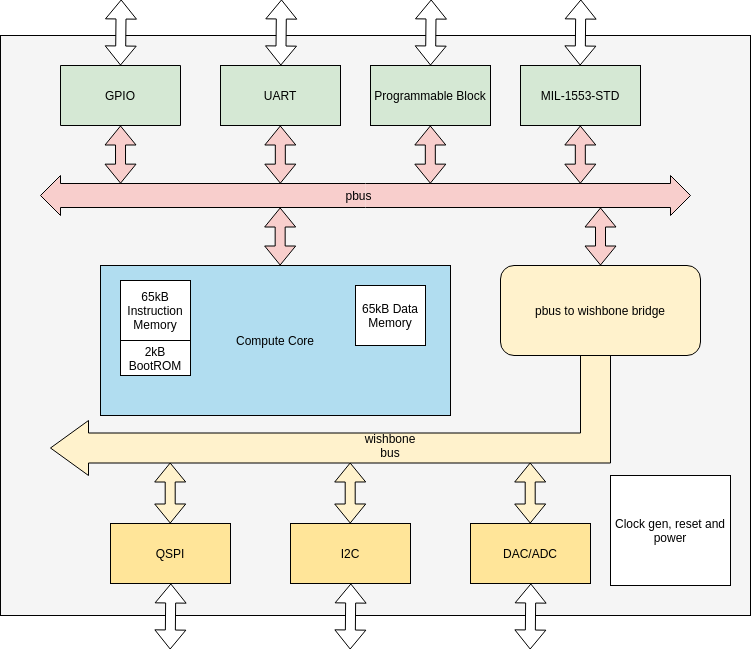
\includegraphics[scale=.35]{nasic2.png}
	\caption{Navigation AISC Base Architecture Block Diagram}
\end{figure}
%\section{Software Architecture}
%\paragraph{\textrm{\textmd{To be Determined}}}
%\section{Communications Architecture}
%\paragraph{\textrm{\textmd{To be Determined}}}
\chapter{Detailed Design}
\section{Compute Core}
\paragraph{\textrm{\textmd{The compute core is a five stage pipled RV-32IM processor as described in previous sections. This chapter illuastrates the functional blocks thatr comprise the core and their functionality.}}}
\subsection{Instruction Fetch stage}
\paragraph{\textrm{\textmd{The Instruction Fetch(IF) stage is tasked with the reading and writing to Instruction memory, Program Counter updtaion and handling of pipeline stalls. Each of these tasks is handled in the following ways:}}}
\begin{enumerate}
	\item The \textbf{PC} register is updated always to increment by a value of 4 (corresponding to the address spcae of 1 32-bit instruction) each clock cycle. This value is used as the fetch address for the instruction memory.The instruction is formed out of the \textbf{dataOut} lines in the instruction memory. The architecture expects a Memory configuration with read latency of one clock cycle.
	\item Due to a read latency of one clock cycle the \textbf{PC} value is stored in anouther register \textbf{PCout}, from where the \textbf{PC} value is fed to the decode stage. Branch and stall operations account for this delay in fetch as well.
	\item Pipeline stalls require atleast two clock cycles to load the output of the stage, hence all stalls will be a minimum of two clock cycles. during these the output instruction is an 'nop' instruction or 0x00000013.
\end{enumerate}
\begin{figure}[h]
	\centering
	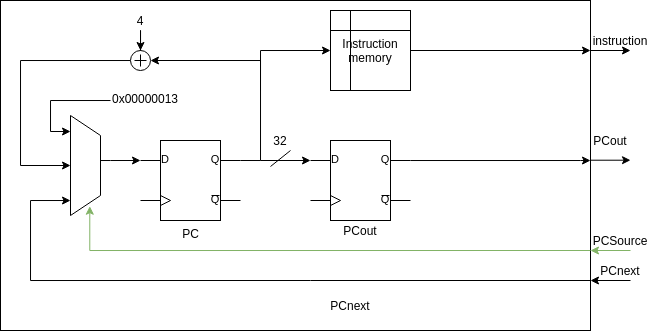
\includegraphics[scale=.45]{ifstage.png}
	\caption{Instruction Stage Block Schematic}
	\label{fig:ifstage}
\end{figure}
\paragraph{\textrm{\textmd{A block schematic is illustrated in Fig.\ref{fig:ifstage}.The IF stage can be programmed for debugging using  the first of two programming ports. The programming is done by halting the pipeline using the \textbf{io\_halt} line. The second read write port is mapped to a higher read address than the data memory. Refer memory map and archuitecture for more details.}}}
\subsection{Execution Stage}
\paragraph{\textrm{\textmd{The Execution stage is, as the name implies, tasked with the execution of the instruction. The functional block diagram of the Stage is given in Fig.\ref{fig:exstage}.  }}}
\begin{figure}[h]
	\centering
	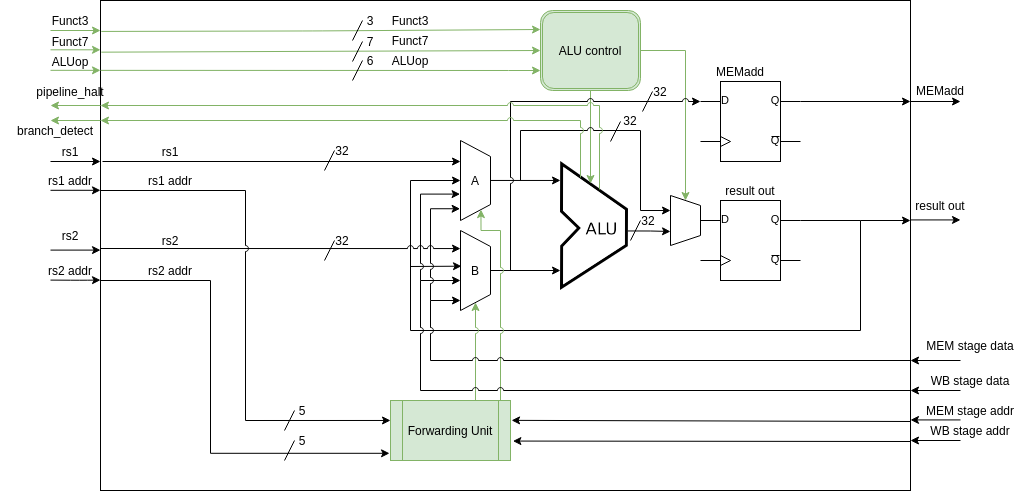
\includegraphics[scale=.35]{exstage.png}
	\caption{Execution Stage Block Schematic}
	\label{fig:exstage}
\end{figure}
\subsubsection{ALU}
\paragraph{\textrm{\textmd{As per the requirements of the Compute core as described in the previous chapters, it is clear that an effective ALU must be simple, and support maximum hardware opeartions with minimal hardware utilization. Hence each possible opeartion the ALU can perform in hardware directly through a behavioural model is given a unique identifier signified by the bits of the \textbf{ALUctl} signal except the Most significant bit and secod-most significant bit. These bits explicitly describe the suboperation on the hardware to be performed. For example  MUL, MULH, MULHSU and MULHU share the same \textbf{ALUctl[4:0]} value of 0101. The operations and their corresponding \textbf{ALUctl} values are summarized in Table~\ref{tab:alu}}}}
\begin{table}[h!t]
	\centering
\begin{tabular}{|c|c|}
		\hline
		\rowcolor[HTML]{34CDF9} 
		Operation & ALUctl \\ [1.5ex] \hline 
		and       & 000000 \\ \hline
		or        & 000001 \\ \hline
		xor       & 000010 \\ \hline
		lt        & 000011 \\ \hline
		ltu       & 010011 \\ \hline
		add       & 000100 \\ \hline
		sub       & 010100 \\ \hline
		mul       & 000101 \\ \hline
		mulh      & 100101 \\ \hline
		mulhu     & 110101 \\ \hline
		mulhsu    & 010101 \\ \hline
		div       & 000110 \\ \hline
		divu      & 010110 \\ \hline
		rem       & 000111 \\ \hline
		remu      & 010111 \\ \hline
		sll       & 001000 \\ \hline
		srl       & 011000 \\ \hline
		sra       & 111000 \\ \hline
\end{tabular}
	\caption{ALU Operations with their corresponfing ALUctl line values}
	\label{tab:alu}
\end{table}

\subsubsection{ALUControl}

\begin{table}[!ht]
	\centering
\begin{tabular}{|c|c|c|c|c|c|c|}
		\hline
		\rowcolor[HTML]{34CDF9} 
		\multicolumn{1}{|l|}{\cellcolor[HTML]{34CDF9}Instr-type} & OPCode & ALUop & Funct7  & Funct3 & ALUctl & ALUOperation \\ [0.5ex] \hline
		U                                                              & LUI                & 0000  & XXXXXXX & XXX    & 000100 & add          \\ \hline
		U                                                              & AUIPC              & 0001  & XXXXXXX & XXX    & 000100 & add          \\ \hline
		UJ                                                             & JAL                & 0010  & XXXXXXX & XXX    & 000100 & add          \\ \hline
		I                                                              & JALR               & 0011  & XXXXXXX & XXX    & 000100 & add          \\ \hline
		Branch(S-type)                                                 & BEQ                & 0100  & XXXXXXX & 000    & 010100 & sub          \\ \hline
		Branch(S-type)                                                 & BNE                & 0100  & XXXXXXX & 001    & 010100 & sub          \\ \hline
		Branch(S-type)                                                 & BLT                & 0100  & XXXXXXX & 100    & 000011 & lt           \\ \hline
		Branch(S-type)                                                 & BGE                & 0100  & XXXXXXX & 101    & 000011 & lt           \\ \hline
		Branch(S-type)                                                 & BLTU               & 0100  & XXXXXXX & 110    & 010011 & ltu          \\ \hline
		Branch(S-type)                                                 & BGEU               & 0100  & XXXXXXX & 111    & 010011 & ltu          \\ \hline
		I                                                              & LB                 & 0101  & XXXXXXX & 000    & 000100 & add          \\ \hline
		I                                                              & LH                 & 0101  & XXXXXXX & 001    & 000100 & add          \\ \hline
		I                                                              & LW                 & 0101  & XXXXXXX & 010    & 000100 & add          \\ \hline
		S                                                              & SB                 & 1000  & XXXXXXX & 000    & 000100 & add          \\ \hline
		S                                                              & SH                 & 1000  & XXXXXXX & 001    & 000100 & add          \\ \hline
		S                                                              & SW                 & 1000  & XXXXXXX & 010    & 000100 & add          \\ \hline
		I                                                              & ADDI               & 0111  & XXXXXXX & 000    & 000100 & add          \\ \hline
		I                                                              & SLTI               & 0111  & XXXXXXX & 010    & 000011 & lt           \\ \hline
		I                                                              & SLTUI              & 0111  & XXXXXXX & 011    & 010011 & ltu          \\ \hline
		I                                                              & XORI               & 0111  & XXXXXXX & 100    & 000010 & xor          \\ \hline
		I                                                              & ORI        & 0111  & XXXXXXX & 110    & 000001 & or           \\ \hline
		I                                                              & ANDI               & 0111  & XXXXXXX & 111    & 000000 & and          \\ \hline
		I                                                              & SLLI               & 0111  & 0000000 & 001    & 001000 & sll          \\ \hline
		I                                                              & SRLI               & 0111  & 0000000 & 101    & 011000 & srl          \\ \hline
		I                                                              & SRAI               & 0111  & 0100000 & 101    & 111000 & sra          \\ \hline
		R                                                              & ADD                & 0110  & 0000000 & 000    & 000100 & add          \\ \hline
		R                                                              & SUB                & 0110  & 0100000 & 000    & 010100 & sub          \\ \hline
		R                                                              & SLL                & 0110  & 0000000 & 001    & 001000 & sll          \\ \hline
		R                                                              & SLT                & 0110  & 0000000 & 010    & 000011 & lt           \\ \hline
		R                                                              & SLTU               & 0110  & 0000000 & 011    & 010011 & ltu          \\ \hline
		R                                                              & XOR                & 0110  & 0000000 & 100    & 000010 & xor          \\ \hline
		R                                                              & SRL                & 0110  & 0000000 & 101    & 011000 & srl          \\ \hline
		R                                                              & SRA                & 0110  & 0100000 & 101    & 111000 & sra          \\ \hline
		R                                                              & OR                 & 0110  & 0000000 & 110    & 000001 & or           \\ \hline
		R                                                              & AND                & 0110  & 0000000 & 111    & 000000 & and          \\ \hline
\end{tabular}
	\caption{Intruction decode sequence(pto)}
	\label{tab:aluctl(a)}
\end{table}                                                         
\begin{table}[!ht]
\centering
\begin{tabular}{|c|c|c|c|c|c|c|}
		\hline
		\rowcolor[HTML]{34CDF9} 
		\multicolumn{1}{|l|}{\cellcolor[HTML]{34CDF9}Instr-type} & OPCode & ALUop & Funct7  & Funct3 & ALUctl & ALUOperation \\ [1ex] \hline
		R                                                              & MUL                & 0110  & 0000001 & 000    & 000101 & mul          \\ \hline
		R                                                              & MULH               & 0110  & 0000001 & 001    & 100101 & mulh         \\ \hline
		R                                                              & MULHU              & 0110  & 0000001 & 010    & 110101 & mulhu        \\ \hline
		R                                                              & MULHSU             & 0110  & 0000001 & 011    & 010101 & mulhsu       \\ \hline
		R                                                              & DIV                & 0110  & 0000001 & 100    & 000110 & div          \\ \hline
		R                                                              & DIVU               & 0110  & 0000001 & 101    & 010110 & divu         \\ \hline
		R                                                              & REM                & 0110  & 0000001 & 110    & 000111 & rem          \\ \hline
		R                                                              & REMU               & 0110  & 0000001 & 111    & 010111 & remu         \\ \hline
\end{tabular}
	\caption{Intruction decode sequence(contd..)}
	\label{tab:aluctl(b)}
\end{table}
\paragraph{\textrm{\textmd{The \textbf{ALUctl} values specified in Table~\ref{tab:alu} can be used in conjunction with the RISCV instruction set user level encoding to generate a truth table for a peice of logic called the ALUControl. This Logic is tasked with decode the operation the ALU has to perform based on the Operation type specified by instruction using a signal generated by the Control Logic and additional Funct7 and Funct3 bits. this decoding is summarized in Tables ~\ref{tab:aluctl(a)} and ~\ref{tab:aluctl(b)}}}}
\paragraph{\textrm{\textmd{Using the information in Table~\ref{tab:aluctl} the values for all insputs for which each output bit of the \textbf{ALUctl} values can be extracted and the following output equations can be derived, assuming \textbf{ALUop} is represented by \textbf{a}, \textbf{Funct7} by \textbf{f} and \textbf{Funct3} by \textbf{b} as shown by Equations~\ref{eq:aluctl0} to ~\ref{eq:aluctl5}. They are heuristically reduced to a minimum size and implemented using a purely combinational circuit using gate based logic and it behaviourally.}}}

\begin{equation}
\begin{aligned}
ALUctl[0] =  & a_3'a_2a_1'a_0'b_2 + a_3'a_2a_1a_0b_2'b_1 + a_3'a_2a_1a_0b_2b_1b_0' +  \\
& a_3'a_2a_1a_0'f_6'f_5'f_4'f_3'f_2'f_1'f_0'b_2'b_1 \\ 
&+ a_3'a_2a_1a_0'f_6'f_5'f_4'f_3'f_2'f_1'f_0'b_2b_1b_0' \\
& +a_3'a_2a_1a_0'f_6'f_5'f_4'f_3'f_2'f_1'f_0b_2'b_1' + a_3'a_2a_1a_0'f_6'f_5'f_4'f_3'f_2'f_1'f_0b_1 
\end{aligned}
\label{eq:aluctl0}
\end{equation}

\begin{equation}
\begin{aligned}
ALUctl[1] = & a_3'a_2a_1'a_0'b_2 + a_3'a_2a_1a_0b_2'b_1 + \\
&  a_3'a_2a_1a_0b_2b_1'b_0' + a_3'a_2a_1a_0'f_6'f_5'f_4'f_3'f_2'f_1'f_0'b_2'b_1 + \\
& a_3'a_2a_1a_0'f_6'f_5'f_4'f_3'f_2'f_1'f_0'b_2b_1'b_0' + a_3'a_2a_1a_0'f_6'f_5'f_4'f_3'f_2'f_1'f_0b_2
\end{aligned}
\label{eq:aluctl1}
\end{equation}

\begin{equation}
\begin{aligned}
ALUctl[2] = & a_3'a_2' + a_3'a_2a_1b_2'b_1' + a_3'a_2a_1'a_0b_2'b_1b_0' 
+ a_3'a_2a_1'a_0b_2b_1' \\
&+ a_3 a_2'a_1'a_0'b_2'b_1' + a_3a_2'a_1'a_0'b_2'b_1b_0'  + a_3'a_2a_1a_0b_2'b_1'b_0'\\
& + a_3'a_2a_1a_0'f_6f_4'f_3'f_2'f_1'f_0'b_2'b_1'b_0'  + a_3'a_2a_1a_0'f_6'f_5'f_4'f_3'f_2'f_1'f_0
\end{aligned}
\label{eq:aluctl2}
\end{equation}

\begin{equation}
\begin{aligned}
ALUctl[3] = & a_3'a_2a_1f_6'f_5'f_4'f_3'f_2'f_1'f_0'b_2'b_1'b_0 + a_3'a_2a_1f_6'f_4'f_3'f_2'f_1'f_0'b_2b_1'b_0
\end{aligned}
\label{eq:aluctl3}
\end{equation}
\begin{equation}
\begin{aligned}
ALUctl[4] = & a_3'a_2a_1'a_0'b_2'b_1' + a_3'a_2a_1'a_0'b_2b_1 + 
a_3'a_2a_1a_0b_2b_1b_0 +\\
& a_3'a_2a_1a_0f_6'f_4'f_3'f_2'f_1'f_0'b_2b_1'b_0 + 
a_3'a_2a_1a_0'f_6'f_5'f_4'f_3'f_2'f_1'f_0'b_2'b_1'b_0' +\\
&  a_3'a_2a_1a_0'f_6'f_5'f_4'f_3'f_2'f_1'f_0'b_2'b_1b_0 + 
a_3'a_2a_1a_0'f_6'f_4'f_3'f_2'f_1'f_0'b_2b_1'b_0' +\\
&  a_3'a_2a_1a_0'f_6'f_5'f_4'f_3'f_2'f_1'f_0b_2'b_1 +  a_3'a_2a_1a_0'f_6'f_5'f_4'f_3'f_2'f_1'f_0b_2b_0
\end{aligned}
\label{eq:aluctl4}
\end{equation}
\begin{equation}
\begin{aligned}
ALUctl[5] =  a_3'a_2a_1a_0'f_6'f_5'f_4'f_3'f_2'f_1'f_0b_2'b_0 +  a_3'a_2a_1f_6'f_5f_4'f_3'f_2'f_1'f_0'b_2b_1'b_0
\end{aligned}
\label{eq:aluctl5}
\end{equation}
\subsubsection{Forwarding Unit}
\paragraph{\textrm{\textmd{The forwarding unit is tasked with ensuring that back-toback instructions that write and read to the same memmory location and/or the same register is handled smoothly in the pipeline. It functions by routing values from subsequent pipeline stages. Under these considerations three possible forwarding paths come up that the Forwarding Unit has to support. These are:}}}
\begin{itemize}
	\item When a previously computed output value becomes the current input argument to the ALU
	\item When the destination register of the Memmory Fetch stage is the argument of the subsequent ALU operation.
	\item When a a register who is being written to in the Write Back stage is the argument for a simultaneous ALU operation.
\end{itemize}
\subsubsection{Branch Detection}
\paragraph{\textrm{\textmd{The branch detection Unit is tasked with Confirming that a Branch condition is valid and the branch can be taken. The Branch Predictors prediction is compared and the pipeline is stalled if the they disagree. The branch detction Unit is tasked with making sense of the condition for operations complementary to the Operations supported by the ALU. For example, the sub operation is used to identify wether two registers are equal in case of a BEQ(branch if Equal)instruction by just checking if the output of the ALU is zero, if not,  the  brach is dropped. The Logical Inverse of this operation is required for the BNE(Branch if Not Equal) instruction. This can be achieved by inverting the implications of the compare. If the ouput of the ALU is zero then the branch is dropped, else if the output is non-zero thenthe branch is taken. This can be extended to complementary Operational pairs like BLT and BGE (Branch if Less than and Branch of Greater than or Equal respectively) }}}


%\paragraph{\textrm{\textmd{This is also a paragraph to remove}}}
%\section{Software Detailed Design}
%\paragraph{\textrm{\textmd{To be Determined}}}
%\chapter{External Interface Design}
%\section{Interface Architecture}
%\paragraph{\textrm{\textmd{To be Determined}}}
%\section{Interface Detailed Design}
%\paragraph{\textrm{\textmd{To be Determined}}}
\section{WISHBONE Bus}
\paragraph{\textrm{\textmd{The WISHBONE System-on-Chip (SOC) Interconnection is a method for	connecting IP cores together to form integrated circuits. Open core SOC design methodology utilizes WISHBONE bus interface to foster design reuse by alleviating	system-on-chip integration problems. With use of this standardize bus interface it is much easier to connect the cores, and therefore much easier to create a custom System-on-Chip.}}}
\paragraph{\textrm{\textmd{This way of SOC design improves the portability and reliability of the system, and results in faster time-to-market for the end user. The objective behind WISHBONE is to create a portable interface that supports both FPGA and ASIC that is independent of the 	semiconductor technology and WISHBONE interfaces should be independent of logic signaling levels.}}}
\begin{figure}[h]
	\centering
	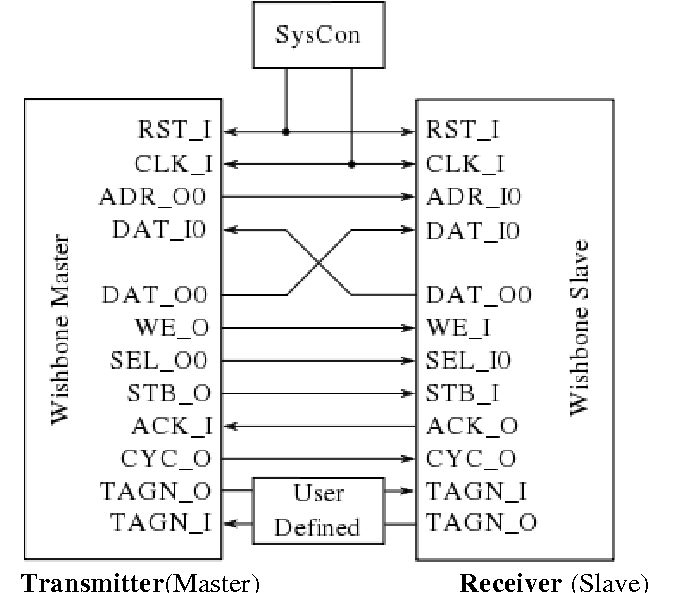
\includegraphics[scale=.4]{interface.png}
	\caption{Wishbone Bus Interface}
	\label{fig:interface}
\end{figure} 		
\paragraph{\textrm{\textmd{Another important reason is to create a flexible interconnection scheme
			that is independent of the type of IP core delivery (Hard, Soft IP) method. The next
			reasons are to have a standard interface that can be written using any hardware
			description language such as VHDL and VERILOG. It supports a variety of bus
			transfer cycle in which the data transaction is independent of the application specific
			functions of the IP cores. It also supports different types of interconnection architectures
			with theoretically infinite range of operating frequency. The final objective of
			WISHBONE bus is that it is absolutely free to use by developers without paying any fee
			for the cores available.}}}
\subsection{WISHBONE Basics }
\begin{figure}[h]
	\centering
	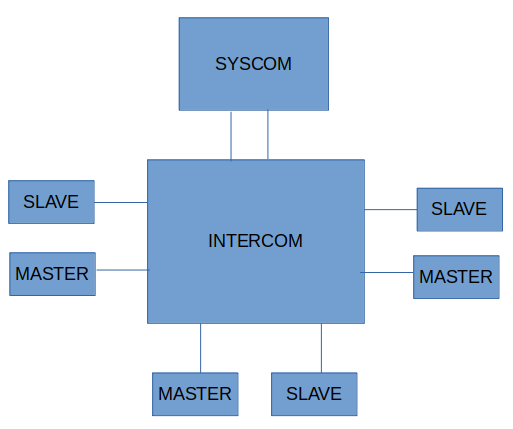
\includegraphics[scale=.6]{wb.png}
	\caption{Interconnection System}
	\label{fig:wb}
\end{figure}
\paragraph{\textrm{\textmd{WISHBONE utilizes “Master” and “Slave” architectures which are connected to
			each other through an interface called “Intercon”. Master is an IP core that initiates the
			data transaction to the SLAVE IP core.Master starts transaction providing an address and control signal to Slave. Slave
			in turn responds to the data transaction with the Master with the specified address range.The Intercon is the medium consists of wires and logics which help in data transfer
			between Master and Slave. The Intercon also requires a “SYSCON” module which
			generates WISHBONE reset and clock signal for the proper functioning of the system.
			Figure:4.4 show the WISHBONE Intercon system which consists of Masters and Slaves
			and SYSCON modules. WISHBONE Intercon can be designed to operate over an infinite
			frequency range. This is called as variable time specification. The speed of the operation
			is only limited by the technology of the integrated circuits. The interconnection can be
			described using hardware description languages like VHDL and Verilog, and the
			system integrator can modify the interconnection according to the requirement of the
			design. Hence WISHBONE interface is different from traditional microcomputer buses
			such as PCI, VME bus and ISA bus. }}}
\subsection{WISHBONE Features }
\paragraph{\textrm{\textmd{The WISHBONE interconnection makes System-on-Chip and design reuse easy by creating a
			standard data exchange protocol. Features of this technology include: }}}
\begin{enumerate}
	\item Simple, compact, logical IP core hardware interfaces that require very few logic gates. 
	\item Variable core interconnection methods support point-to-point, shared bus, crossbar
	switch, and switched fabric interconnections. 
	\item Handshaking protocol allows each IP core to throttle its data transfer speed.
	\item Supports single clock data transfers. 
	\item MASTER / SLAVE architecture for very flexible system designs. 
	\item Synchronous design assures portability, simplicity and ease of use. 
	\item Independent of hardware technology (FPGA, ASIC, etc.). 
\end{enumerate}
\paragraph{\textrm{\textmd {The WISHBONE specification regulates the ordering of data. This is because data can be presented in two different ways. In the first way, the most significant byte of an operand is placed
			at the higher (bigger) address. In the second way, the most significant byte of an operand can be
			placed at the lower (smaller) address. These are called BIG ENDIAN and LITTLE ENDIAN
			data operands, respectively. WISHBONE supports both types.  }}}
\section{MIL STD 1553}
\begin{figure}[h]
	\centering
	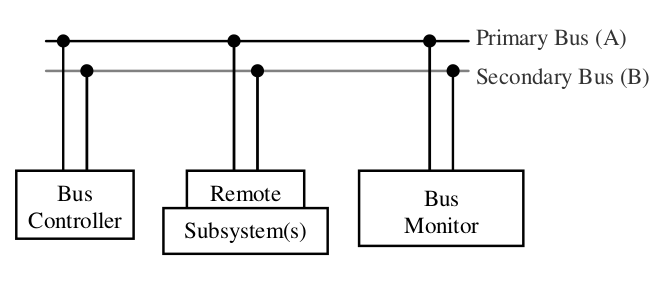
\includegraphics[scale=.4]{1553.png}
	\caption{MIL STD 1553}
	\label{fig:1553}
\end{figure}
\paragraph{\textrm{\textmd{The Hardware elements of	MIL-STD-1553 BUS consist of the data bus and terminals. The three terminals are:}}}
\begin{enumerate}
	\item Bus controller (BC)
	\item Remote terminal(RT)/Remote Subsystems
	\item Bus Monitor Terminal (MT)
\end{enumerate} 
\subparagraph{Remote Terminal}
\paragraph{\textrm{\textmd{A remote terminal typically consists of a transceiver, an encoder/decoder,
			a protocol controller, a buffer or memory, and a subsystem interface. In a
			modern black box containing a computer or processor, the subsystem
			interface may consist of the buffers and logic necessary to interface to the
			computer's address, data, and control buses. For dual redundant systems,
			the most prevalent in today's applications, two transceivers and two encod-
			ers/decoders would be required.It should be pointed out that if
			the remote terminal shares common memory (verses private), then that
			portion of the memory that the remote terminal can address should be
			considered part of the remote terminal.The
			remote terminal consists of all the electronics necessary to transfer data between the data bus and the user or originator of the data being
			transferred.}}}
\begin{figure}[h]
	\centering
	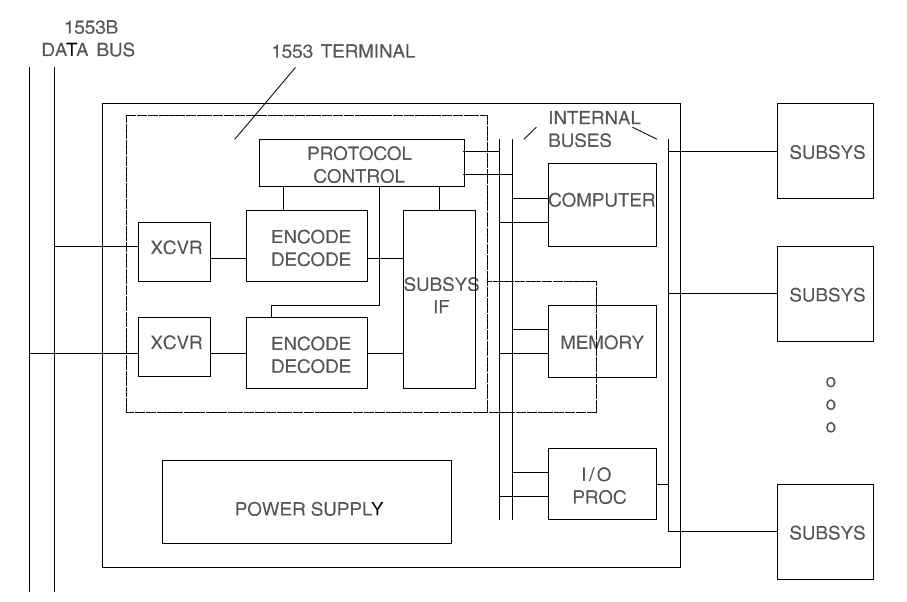
\includegraphics[scale=.4]{rt.png}
	\caption{Terminal Definition}
	\label{fig:rt}
\end{figure}
\paragraph{\textrm{\textmd{But a remote terminal must be more than just a data formatter. It must be
capable of receiving and decoding commands from the bus controller and
responding accordingly. It must also be capable of buffering a message
worth of data, detecting transmission errors and performing validation tests upon the data, and reporting the status of the message transfer. 
A remote terminal must follow the protocol defined by the standard. It can
only respond to commands received from the bus controller. When it receives a valid command, it must respond
within a very small, closely defined amount of time. If a message doesn’t
meet the validity requirements defined, then the remote terminal must
invalidate the message and discard the data. In addition to reporting status to the bus controller, most
remote terminals today are capable of providing some level of status
information to the subsystem.}}}	
\subparagraph{Bus Controller}
\paragraph{\textrm{\textmd{The bus controller is responsible for directing the flow of data on the data
			bus. While several terminals may be capable of performing as the bus
			controller, only one bus controller may be active at a time. The bus
			controller is the only one allowed to issue commands onto the data bus.
			The commands may be for the transfer of data or the control and manage-
			ment of the bus (mode commands).
			Typically, the bus controller is a function that is contained within some
			other computer, such as a mission computer, a display processor, or a fire
			control computer. The complexity of the electronics associated with the
			bus controller is a function of the subsystem interface, the amount of error management and processing to be
			performed, and the architecture of the bus controller.}}}
\subparagraph{Bus Monitor}
\paragraph{\textrm{\textmd{A bus monitor is a terminal that listens (monitors) to the exchange of
information on the data bus. The standard strictly defines how bus
monitors may be used, stating that the information obtained by a bus
monitor be used “for off-line applications (e.g., flight test recording,
maintenance recording or mission analysis) or to provide the back-up bus
controller sufficient information to take over as the bus controller.” A
monitor may collect all the data from the bus or may collect selected data.
The reason for restricting its use is that while a monitor may collect data, it
deviates from the command-response protocol of the standard, in that a
monitor is a passive device that doesn’t transmit a status word and
therefore cannot report on the status of the information transferred. Bus
monitors fall into two categories:}}}
\begin{enumerate}
	\item A recorder for testing.
	\item A terminal functioning as a back-up bus controller.
\end{enumerate} 
\paragraph{\textrm{\textmd{In collecting data, a monitor must perform the same message validation
functions as the remote terminal and if an error is detected, inform the
subsystem of the error (the subsystem may still record the data, but the
error should be noted). For monitors, which function as recorders for
testing, the subsystem is typically a recording device such as a magnetic
tape or disk, or a telemetry transmitter. For monitors, which function as
back-up bus controllers, the subsystem is the computer.
Today it is common for bus monitors to contain a remote terminal. When
the monitor receives a command addressed to its terminal address, it
responds as a remote terminal. For all other commands, it functions as a
monitor. The remote terminal portion can be used to provide feedback to
the bus controller, which monitors status and the amount of memory or
time (i.e. recording tape) left. The remote terminal portion also can be
used to reprogram a selective monitor as to what messages to capture.}}}
\subparagraph{Operation}
\paragraph{\textrm{\textmd{The Standard defines the data bus to be a single path among the bus controller and remote terminals.MIL-STD-1553B defines the data bus structure for interconnection of up to 31 remote terminal (RT) devices.}}}
\paragraph{\textrm{\textmd{ A single controller device on the bus initiates the command/response communication with the remote devices. The remote and control devices are interconnected over two, separate buses.Normal operation involves only the primary bus with the secondary bus available as redundant backup in the event of primary bus damage or failure.The BC is the master device and operating as a bus controller. The BC initiates all theinformation transfers through the data bus. The standard specifies the informationtransfers between RTs to follow a command/response format.The BC sendscommands to the RTs to tell them what to do. The BC can be a separate subsystem or just a portion of a subsystem.The RT is the device interfaces the data bus to the sub-system and transfers data in and out of the subsystem.}}}			
\paragraph{\textrm{\textmd {The RT can be an independent subsystem or it can be portion of the subsystem. The Standard allows for up to 31 RTs in a system.The MT is optional and works like a passive device which examines all data on the bus. It can record all data or selected data for off-line applications}}}
\paragraph{\textrm {MIL-STD-1553 communication uses three word types:}}
\begin{enumerate}
	\item Command
	\item Status
	\item Data
\end{enumerate} 
\paragraph{\textrm{\textmd {All these three words are of 20 bits in length. Three bits out of 20 bits are used for the word sync, 16 bits are used for information and the last one bit is for parity. The sync bit differentiates the data words from command and status words.In addition, mode messages are defined for managing the bus system and error recovery.}}}
\begin{figure}[h]
	\centering
	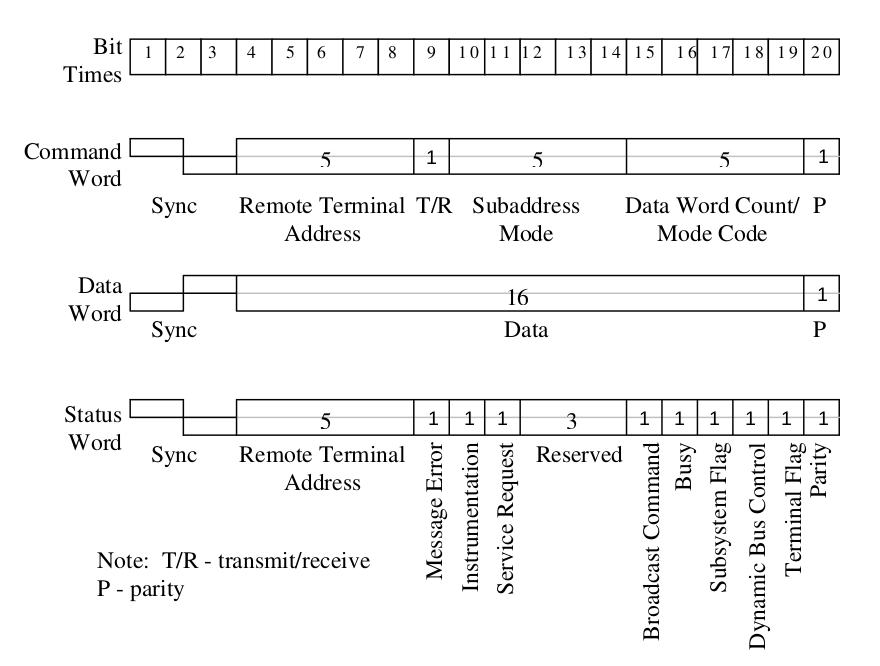
\includegraphics[scale=.35]{word.png}
	\caption{Word Formats}
	\label{fig:word}
\end{figure}
\subsection{Command Word}
\paragraph{\textrm{\textmd{ The BC issues “Command Word (CW)” to RTs to perform specific functions. The CW is shown in the Figure \ref{fig:cmd}.The address field is 5 bit and the BC can address maximum 31 terminals.Command words are issued/transmitted only by the BC. BC directs any RT to transmit, receive or perform a specified action.}}}
\begin{figure}[h]
	\centering
	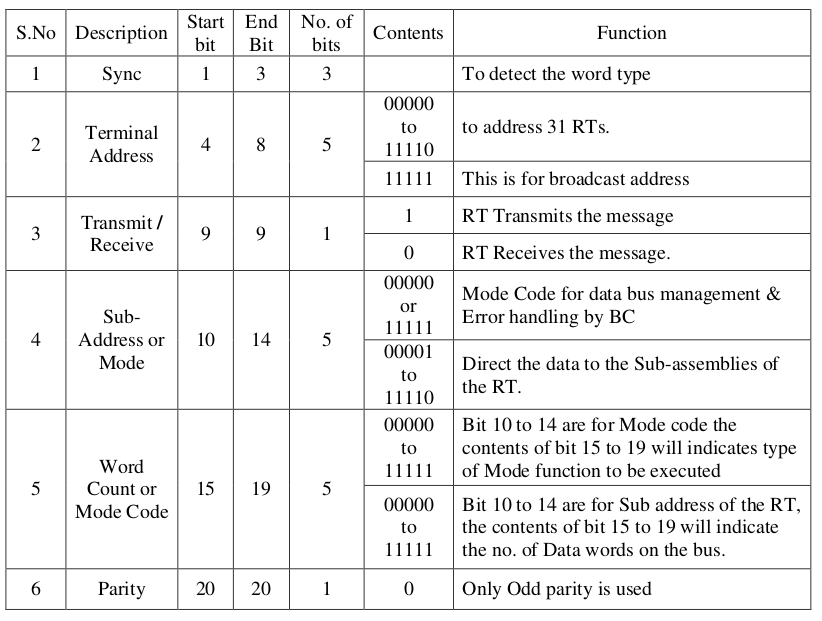
\includegraphics[scale=.4]{command.png}
	\caption{Command Word}
	\label{fig:cmd}
\end{figure}
\subsection{Status Word}
\paragraph{\textrm{\textmd{A Remote terminal( RT)sends Status word in response to BCs command word. The status word is to convey that the transmission is OK or error.The status word is issued/transmitted only by a RT and provides general information on the state of the RT as shown in Figure \ref{fig:sts} }}}
\begin{figure}[h]
	\centering
	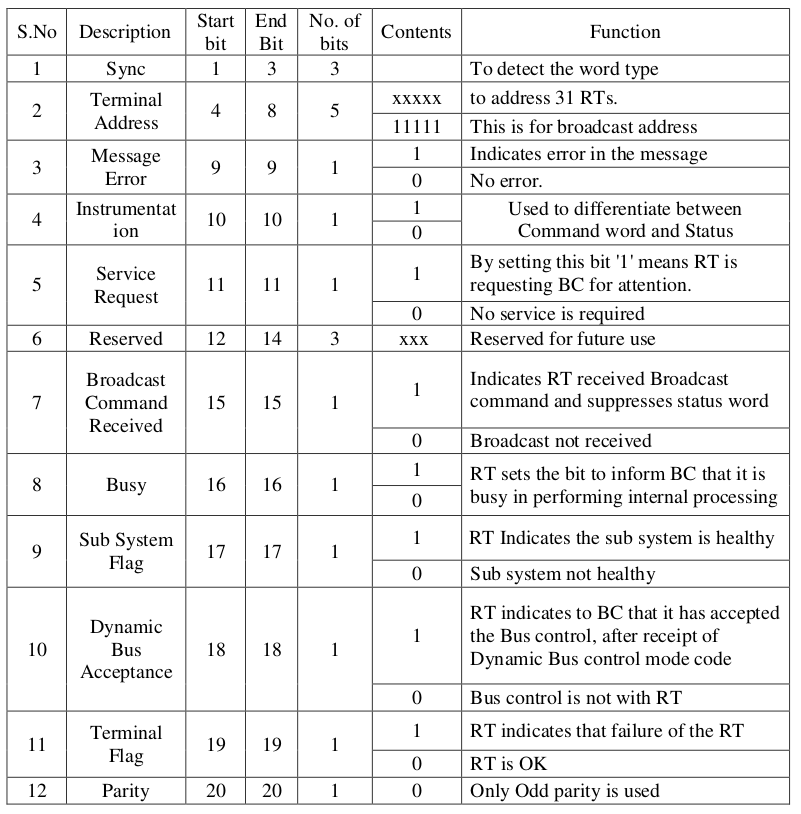
\includegraphics[scale=.4]{status.png}
	\caption{Status Word}
	\label{fig:sts}
\end{figure}
\subsection{Data Word}
\paragraph{\textrm{\textmd{ The Data Word (DW) contains the actual information that is to be transferred within the message.Data words may be transmitted by either the BC or RT.Messages are from BC to RT transfers, RT to BC transfers, and RT to RT transfers.The first three-bits are “data sync” as shown in Figure \ref{fig:data}.}}}
\begin{figure}[h]
	\centering
	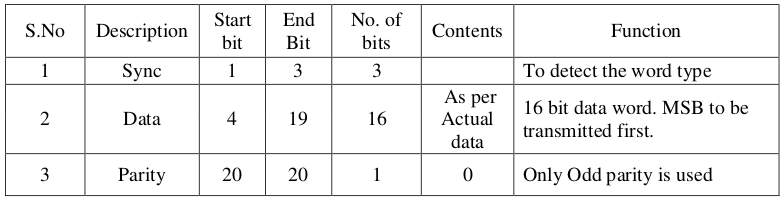
\includegraphics[scale=.4]{data.png}
	\caption{Data Word}
	\label{fig:data}
\end{figure}


\chapter{\large \MakeUppercase{Litreature Survey}}
\chapter{\large \MakeUppercase {Theoretical Analysis and Modelling}}
\chapter{\large \MakeUppercase {Computational Simulation \& verification}}
\chapter{\large \MakeUppercase {Experimental Testing \& Validation}}
\end{document}
